\documentclass[12pt,letterpaper]{article}
\usepackage[letterpaper,left=0.65in,right=0.65in,top=0.76in,bottom=0.67in,headheight=16pt,headsep=14pt,footskip=25pt]{geometry}
\usepackage[T1]{fontenc}
\usepackage{lmodern}
\pdfmapfile{+lm.map}
\usepackage{tikz}
\usepackage{fancyhdr}
\renewcommand{\familydefault}{\sfdefault}
\pagestyle{fancy}
\fancyhf{}
\renewcommand{\headrulewidth}{0pt}
\renewcommand{\footrulewidth}{0pt}
\setlength{\parindent}{0pt}
\setlength{\parskip}{0pt}
\setlength{\emergencystretch}{2em}
\raggedright
\newcommand{\problem}[2]{\textbf{Problem #1:} #2\par}
\newcommand{\recordlines}[1]{\vspace{0.30cm}\foreach \n in {1,...,#1}{\noindent\rule{\linewidth}{0.25pt}\par\vspace{0.72cm}}}

\fancyhead[L]{\fontsize{10.5}{12}\selectfont Week 22 / Meeting regions / Grades 4--5}
\fancyfoot[L]{\fontsize{9}{11}\selectfont Bellingham Math Circle / Week 22 / F22-45-v3}
\fancyfoot[R]{\fontsize{9}{11}\selectfont\thepage}
\begin{document}
\fontsize{13}{17}\selectfont
Use each label once in two groups, with at least one label in each. Draw each group's stretched-band region and lightly shade its inside. Use the centers of the marks. Sharing even one point counts. Swapping the two groups is the same split.\par
\vspace{0.15cm}
\begin{center}
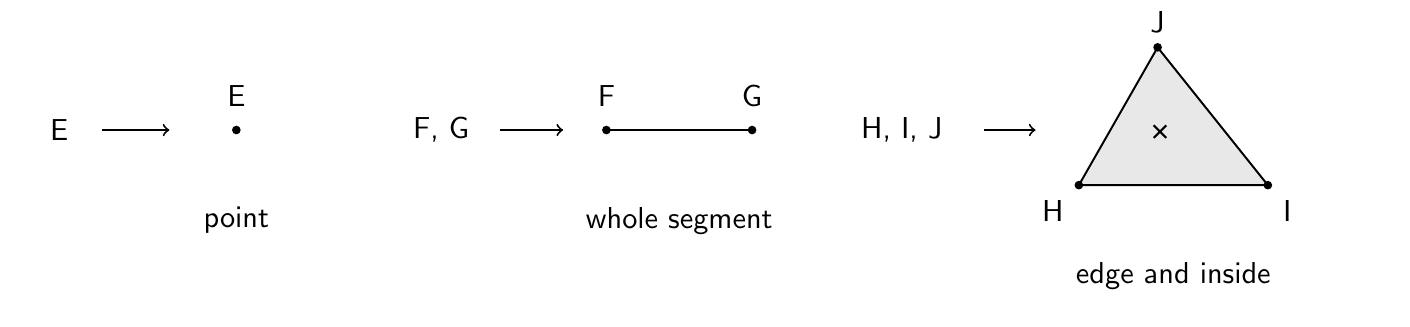
\begin{tikzpicture}[x=1cm,y=1cm,font=\fontsize{11}{13}\selectfont]
\path[use as bounding box] (0,-.65) rectangle (17.2,2.8);
\node at (.4,1.5) {E};
\draw[->,line width=.7pt] (.95,1.5) -- (1.8,1.5);
\fill (2.65,1.5) circle (.055);
\node[above=5pt] at (2.65,1.5) {E};
\node at (2.65,.35) {point};
\node at (5.25,1.5) {F, G};
\draw[->,line width=.7pt] (6,1.5) -- (6.8,1.5);
\draw[line width=1pt] (7.35,1.5) -- (9.2,1.5);
\fill (7.35,1.5) circle (.055);\fill (9.2,1.5) circle (.055);
\node[above=5pt] at (7.35,1.5) {F};\node[above=5pt] at (9.2,1.5) {G};
\node at (8.275,.35) {whole segment};
\node at (11.1,1.5) {H, I, J};
\draw[->,line width=.7pt] (12.15,1.5) -- (12.8,1.5);
\filldraw[fill=black!9,line width=.7pt] (13.35,.8) -- (15.75,.8) -- (14.35,2.55) -- cycle;
\foreach \x/\y in {13.35/.8,15.75/.8,14.35/2.55}{\fill (\x,\y) circle (.055);}
\node[below left=2pt] at (13.35,.8) {H};\node[below right=2pt] at (15.75,.8) {I};\node[above=2pt] at (14.35,2.55) {J};
\draw[line width=.8pt] (14.3,1.40) -- (14.46,1.56) (14.3,1.56) -- (14.46,1.40);
\node at (14.55,-.35) {edge and inside};
\end{tikzpicture}
\end{center}
\vspace{0.15cm}
\problem{1}{Put D on each cross. For each position, split A, B, C, and D so their two regions meet, and mark a shared point.}
\vspace{0.38cm}
\begin{center}
\begin{tikzpicture}[x=1cm,y=1cm]
\path[use as bounding box] (-0.04,-0.04) rectangle (12.64,12.64);
\draw[black!27,line width=0.4pt] (0,0) rectangle (12.6,12.6);
\fill (2,2) circle (0.057cm);
\node[below left=5pt,inner sep=0pt,font=\fontsize{14}{16}\selectfont] at (2,2) {A};
\fill (10.5,3) circle (0.057cm);
\node[below right=5pt,inner sep=0pt,font=\fontsize{14}{16}\selectfont] at (10.5,3) {B};
\fill (4.5,10) circle (0.057cm);
\node[above=5pt,inner sep=0pt,font=\fontsize{14}{16}\selectfont] at (4.5,10) {C};
\draw[line width=0.8pt] (9.710,8.910) -- (9.890,9.090) (9.710,9.090) -- (9.890,8.910);
\draw[line width=0.8pt] (4.910,4.910) -- (5.090,5.090) (4.910,5.090) -- (5.090,4.910);
\draw[line width=0.8pt] (6.160,2.410) -- (6.340,2.590) (6.160,2.590) -- (6.340,2.410);
\draw[line width=0.8pt] (0.910,5.910) -- (1.090,6.090) (0.910,6.090) -- (1.090,5.910);
\end{tikzpicture}
\end{center}
\newpage
\problem{2}{Find every split whose regions meet. Explain how you know your list is complete.}
\vspace{0.38cm}
\begin{center}
\begin{tikzpicture}[x=1cm,y=1cm]
\path[use as bounding box] (-0.04,-0.04) rectangle (12.64,12.64);
\draw[black!27,line width=0.4pt] (0,0) rectangle (12.6,12.6);
\fill (2,3) circle (0.057cm);
\node[below right=5pt,inner sep=0pt,font=\fontsize{14}{16}\selectfont] at (2,3) {A};
\fill (8,9) circle (0.057cm);
\node[below right=5pt,inner sep=0pt,font=\fontsize{14}{16}\selectfont] at (8,9) {B};
\fill (5,6) circle (0.057cm);
\node[below right=5pt,inner sep=0pt,font=\fontsize{14}{16}\selectfont] at (5,6) {C};
\fill (10,11) circle (0.057cm);
\node[below right=5pt,inner sep=0pt,font=\fontsize{14}{16}\selectfont] at (10,11) {D};
\end{tikzpicture}
\end{center}
\recordlines{2}
\newpage
\problem{2}{Find every split whose regions meet. Explain how you know your list is complete.}
\vspace{0.38cm}
\begin{center}
\begin{tikzpicture}[x=1cm,y=1cm]
\begin{scope}[shift={(0.0000,12.3600)},x=0.45238095238095cm,y=0.45238095238095cm]
\draw[black!27,line width=0.4pt] (0,0) rectangle (12.6,12.6);
\fill (2,3) circle (0.045cm);
\node[below right=4pt,inner sep=0pt,font=\fontsize{11}{13}\selectfont] at (2,3) {A};
\fill (8,9) circle (0.045cm);
\node[below right=4pt,inner sep=0pt,font=\fontsize{11}{13}\selectfont] at (8,9) {B};
\fill (5,6) circle (0.045cm);
\node[below right=4pt,inner sep=0pt,font=\fontsize{11}{13}\selectfont] at (5,6) {C};
\fill (10,11) circle (0.045cm);
\node[below right=4pt,inner sep=0pt,font=\fontsize{11}{13}\selectfont] at (10,11) {D};
\end{scope}
\begin{scope}[shift={(6.1800,12.3600)},x=0.45238095238095cm,y=0.45238095238095cm]
\draw[black!27,line width=0.4pt] (0,0) rectangle (12.6,12.6);
\fill (2,3) circle (0.045cm);
\node[below right=4pt,inner sep=0pt,font=\fontsize{11}{13}\selectfont] at (2,3) {A};
\fill (8,9) circle (0.045cm);
\node[below right=4pt,inner sep=0pt,font=\fontsize{11}{13}\selectfont] at (8,9) {B};
\fill (5,6) circle (0.045cm);
\node[below right=4pt,inner sep=0pt,font=\fontsize{11}{13}\selectfont] at (5,6) {C};
\fill (10,11) circle (0.045cm);
\node[below right=4pt,inner sep=0pt,font=\fontsize{11}{13}\selectfont] at (10,11) {D};
\end{scope}
\begin{scope}[shift={(0.0000,6.1800)},x=0.45238095238095cm,y=0.45238095238095cm]
\draw[black!27,line width=0.4pt] (0,0) rectangle (12.6,12.6);
\fill (2,3) circle (0.045cm);
\node[below right=4pt,inner sep=0pt,font=\fontsize{11}{13}\selectfont] at (2,3) {A};
\fill (8,9) circle (0.045cm);
\node[below right=4pt,inner sep=0pt,font=\fontsize{11}{13}\selectfont] at (8,9) {B};
\fill (5,6) circle (0.045cm);
\node[below right=4pt,inner sep=0pt,font=\fontsize{11}{13}\selectfont] at (5,6) {C};
\fill (10,11) circle (0.045cm);
\node[below right=4pt,inner sep=0pt,font=\fontsize{11}{13}\selectfont] at (10,11) {D};
\end{scope}
\begin{scope}[shift={(6.1800,6.1800)},x=0.45238095238095cm,y=0.45238095238095cm]
\draw[black!27,line width=0.4pt] (0,0) rectangle (12.6,12.6);
\fill (2,3) circle (0.045cm);
\node[below right=4pt,inner sep=0pt,font=\fontsize{11}{13}\selectfont] at (2,3) {A};
\fill (8,9) circle (0.045cm);
\node[below right=4pt,inner sep=0pt,font=\fontsize{11}{13}\selectfont] at (8,9) {B};
\fill (5,6) circle (0.045cm);
\node[below right=4pt,inner sep=0pt,font=\fontsize{11}{13}\selectfont] at (5,6) {C};
\fill (10,11) circle (0.045cm);
\node[below right=4pt,inner sep=0pt,font=\fontsize{11}{13}\selectfont] at (10,11) {D};
\end{scope}
\begin{scope}[shift={(0.0000,0.0000)},x=0.45238095238095cm,y=0.45238095238095cm]
\draw[black!27,line width=0.4pt] (0,0) rectangle (12.6,12.6);
\fill (2,3) circle (0.045cm);
\node[below right=4pt,inner sep=0pt,font=\fontsize{11}{13}\selectfont] at (2,3) {A};
\fill (8,9) circle (0.045cm);
\node[below right=4pt,inner sep=0pt,font=\fontsize{11}{13}\selectfont] at (8,9) {B};
\fill (5,6) circle (0.045cm);
\node[below right=4pt,inner sep=0pt,font=\fontsize{11}{13}\selectfont] at (5,6) {C};
\fill (10,11) circle (0.045cm);
\node[below right=4pt,inner sep=0pt,font=\fontsize{11}{13}\selectfont] at (10,11) {D};
\end{scope}
\begin{scope}[shift={(6.1800,0.0000)},x=0.45238095238095cm,y=0.45238095238095cm]
\draw[black!27,line width=0.4pt] (0,0) rectangle (12.6,12.6);
\fill (2,3) circle (0.045cm);
\node[below right=4pt,inner sep=0pt,font=\fontsize{11}{13}\selectfont] at (2,3) {A};
\fill (8,9) circle (0.045cm);
\node[below right=4pt,inner sep=0pt,font=\fontsize{11}{13}\selectfont] at (8,9) {B};
\fill (5,6) circle (0.045cm);
\node[below right=4pt,inner sep=0pt,font=\fontsize{11}{13}\selectfont] at (5,6) {C};
\fill (10,11) circle (0.045cm);
\node[below right=4pt,inner sep=0pt,font=\fontsize{11}{13}\selectfont] at (10,11) {D};
\end{scope}
\end{tikzpicture}
\end{center}
\newpage
\problem{3}{Take turns placing A, B, C, and D in the box. Try to make an arrangement with no successful split. Decide whether your opponent must always be able to find one.}
\vspace{0.38cm}
\begin{center}
\begin{tikzpicture}[x=1cm,y=1cm]
\path[use as bounding box] (-0.04,-0.04) rectangle (12.64,12.64);
\draw[black!27,line width=0.4pt] (0,0) rectangle (12.6,12.6);
\end{tikzpicture}
\end{center}
\recordlines{2}
\newpage
\problem{4}{A and D share a location. Find every split whose regions meet. Does a successful split always exist when two of four labels share a location? Explain.}
\vspace{0.38cm}
\begin{center}
\begin{tikzpicture}[x=1cm,y=1cm]
\path[use as bounding box] (-0.04,-0.04) rectangle (12.64,12.64);
\draw[black!27,line width=0.4pt] (0,0) rectangle (12.6,12.6);
\fill (3,3) circle (0.057cm);
\node[below=6pt,inner sep=0pt,font=\fontsize{14}{16}\selectfont] at (3,3) {A, D};
\fill (10,4.5) circle (0.057cm);
\node[right=6pt,inner sep=0pt,font=\fontsize{14}{16}\selectfont] at (10,4.5) {B};
\fill (5.5,10) circle (0.057cm);
\node[above=6pt,inner sep=0pt,font=\fontsize{14}{16}\selectfont] at (5.5,10) {C};
\end{tikzpicture}
\end{center}
\recordlines{2}
\newpage
\problem{4}{A and D share a location. Find every split whose regions meet. Does a successful split always exist when two of four labels share a location? Explain.}
\vspace{0.38cm}
\begin{center}
\begin{tikzpicture}[x=1cm,y=1cm]
\begin{scope}[shift={(0.0000,12.3600)},x=0.45238095238095cm,y=0.45238095238095cm]
\draw[black!27,line width=0.4pt] (0,0) rectangle (12.6,12.6);
\fill (3,3) circle (0.045cm);
\node[below=4pt,inner sep=0pt,font=\fontsize{11}{13}\selectfont] at (3,3) {A, D};
\fill (10,4.5) circle (0.045cm);
\node[right=4pt,inner sep=0pt,font=\fontsize{11}{13}\selectfont] at (10,4.5) {B};
\fill (5.5,10) circle (0.045cm);
\node[above=4pt,inner sep=0pt,font=\fontsize{11}{13}\selectfont] at (5.5,10) {C};
\end{scope}
\begin{scope}[shift={(6.1800,12.3600)},x=0.45238095238095cm,y=0.45238095238095cm]
\draw[black!27,line width=0.4pt] (0,0) rectangle (12.6,12.6);
\fill (3,3) circle (0.045cm);
\node[below=4pt,inner sep=0pt,font=\fontsize{11}{13}\selectfont] at (3,3) {A, D};
\fill (10,4.5) circle (0.045cm);
\node[right=4pt,inner sep=0pt,font=\fontsize{11}{13}\selectfont] at (10,4.5) {B};
\fill (5.5,10) circle (0.045cm);
\node[above=4pt,inner sep=0pt,font=\fontsize{11}{13}\selectfont] at (5.5,10) {C};
\end{scope}
\begin{scope}[shift={(0.0000,6.1800)},x=0.45238095238095cm,y=0.45238095238095cm]
\draw[black!27,line width=0.4pt] (0,0) rectangle (12.6,12.6);
\fill (3,3) circle (0.045cm);
\node[below=4pt,inner sep=0pt,font=\fontsize{11}{13}\selectfont] at (3,3) {A, D};
\fill (10,4.5) circle (0.045cm);
\node[right=4pt,inner sep=0pt,font=\fontsize{11}{13}\selectfont] at (10,4.5) {B};
\fill (5.5,10) circle (0.045cm);
\node[above=4pt,inner sep=0pt,font=\fontsize{11}{13}\selectfont] at (5.5,10) {C};
\end{scope}
\begin{scope}[shift={(6.1800,6.1800)},x=0.45238095238095cm,y=0.45238095238095cm]
\draw[black!27,line width=0.4pt] (0,0) rectangle (12.6,12.6);
\fill (3,3) circle (0.045cm);
\node[below=4pt,inner sep=0pt,font=\fontsize{11}{13}\selectfont] at (3,3) {A, D};
\fill (10,4.5) circle (0.045cm);
\node[right=4pt,inner sep=0pt,font=\fontsize{11}{13}\selectfont] at (10,4.5) {B};
\fill (5.5,10) circle (0.045cm);
\node[above=4pt,inner sep=0pt,font=\fontsize{11}{13}\selectfont] at (5.5,10) {C};
\end{scope}
\begin{scope}[shift={(0.0000,0.0000)},x=0.45238095238095cm,y=0.45238095238095cm]
\draw[black!27,line width=0.4pt] (0,0) rectangle (12.6,12.6);
\fill (3,3) circle (0.045cm);
\node[below=4pt,inner sep=0pt,font=\fontsize{11}{13}\selectfont] at (3,3) {A, D};
\fill (10,4.5) circle (0.045cm);
\node[right=4pt,inner sep=0pt,font=\fontsize{11}{13}\selectfont] at (10,4.5) {B};
\fill (5.5,10) circle (0.045cm);
\node[above=4pt,inner sep=0pt,font=\fontsize{11}{13}\selectfont] at (5.5,10) {C};
\end{scope}
\begin{scope}[shift={(6.1800,0.0000)},x=0.45238095238095cm,y=0.45238095238095cm]
\draw[black!27,line width=0.4pt] (0,0) rectangle (12.6,12.6);
\fill (3,3) circle (0.045cm);
\node[below=4pt,inner sep=0pt,font=\fontsize{11}{13}\selectfont] at (3,3) {A, D};
\fill (10,4.5) circle (0.045cm);
\node[right=4pt,inner sep=0pt,font=\fontsize{11}{13}\selectfont] at (10,4.5) {B};
\fill (5.5,10) circle (0.045cm);
\node[above=4pt,inner sep=0pt,font=\fontsize{11}{13}\selectfont] at (5.5,10) {C};
\end{scope}
\end{tikzpicture}
\end{center}
\newpage
\problem{5}{Make two four-dot arrangements that each have exactly one successful split, with different successful splits. Make a third arrangement with more than one successful split. Explain how you checked the number of successful splits.}
\vspace{0.38cm}
\begin{center}
\begin{tikzpicture}[x=1cm,y=1cm]
\path[use as bounding box] (-0.04,-0.04) rectangle (12.64,12.64);
\draw[black!27,line width=0.4pt] (0,0) rectangle (12.6,12.6);
\end{tikzpicture}
\end{center}
\recordlines{2}
\newpage
\problem{5}{Make two four-dot arrangements that each have exactly one successful split, with different successful splits. Make a third arrangement with more than one successful split. Explain how you checked the number of successful splits.}
\vspace{0.38cm}
\begin{center}
\begin{tikzpicture}[x=1cm,y=1cm]
\path[use as bounding box] (-0.04,-0.04) rectangle (12.64,12.64);
\draw[black!27,line width=0.4pt] (0,0) rectangle (12.6,12.6);
\end{tikzpicture}
\end{center}
\recordlines{2}
\newpage
\problem{5}{Make two four-dot arrangements that each have exactly one successful split, with different successful splits. Make a third arrangement with more than one successful split. Explain how you checked the number of successful splits.}
\vspace{0.38cm}
\begin{center}
\begin{tikzpicture}[x=1cm,y=1cm]
\path[use as bounding box] (-0.04,-0.04) rectangle (12.64,12.64);
\draw[black!27,line width=0.4pt] (0,0) rectangle (12.6,12.6);
\end{tikzpicture}
\end{center}
\recordlines{2}
\newpage
\problem{6}{Can every arrangement of A, B, C, and D be split into two groups whose regions meet? Give an explanation that covers all arrangements, including dots in a straight line and labels at the same point.}
\vspace{0.38cm}
\begin{center}
\begin{tikzpicture}[x=1cm,y=1cm]
\path[use as bounding box] (-0.04,-0.04) rectangle (12.64,12.64);
\draw[black!27,line width=0.4pt] (0,0) rectangle (12.6,12.6);
\end{tikzpicture}
\end{center}
\recordlines{3}
\newpage
\problem{7}{Can these three dots be split into two groups whose regions meet? Explain why your answer covers every split. Find the smallest number of dots that guarantees a successful split for every arrangement, and explain why fewer cannot give that guarantee.}
\vspace{0.38cm}
\begin{center}
\begin{tikzpicture}[x=1cm,y=1cm]
\path[use as bounding box] (-0.04,-0.04) rectangle (12.64,12.64);
\draw[black!27,line width=0.4pt] (0,0) rectangle (12.6,12.6);
\fill (2,3) circle (0.057cm);
\node[below left=5pt,inner sep=0pt,font=\fontsize{14}{16}\selectfont] at (2,3) {A};
\fill (10.3,4) circle (0.057cm);
\node[below right=5pt,inner sep=0pt,font=\fontsize{14}{16}\selectfont] at (10.3,4) {B};
\fill (4.8,10.1) circle (0.057cm);
\node[above=5pt,inner sep=0pt,font=\fontsize{14}{16}\selectfont] at (4.8,10.1) {C};
\end{tikzpicture}
\end{center}
\recordlines{2}
\end{document}
